% Running Header
\noindent
{\small\sffamily\bfseries MỤC 2.2}\quad {\small\sffamily Giới hạn của hàm số}\hfill {\small\sffamily\bfseries 83}
\vspace{16pt}

% Section Title with decorative lines in margin
\noindent\llap{%
  
\begin{tikzpicture}[baseline=-0.3ex]
    \foreach \i in {-2, -1, 0, 1, 2} {
      \draw[cyan!75!blue, line width=0.65pt] (-3.8, \i*2.8pt) -- (-0.8, \i*2.8pt);
    }
  \end{tikzpicture}\hspace{0.35cm}%
  {\color{cyan!75!blue}\fontsize{22}{26}\selectfont\sffamily\bfseries 2.2}%
  \hspace{0.25cm}%
  {\color{cyan!75!blue}\rule[-0.25ex]{1.2pt}{1.3em}}%
  \hspace{0.35cm}%
}%
{\fontsize{19}{23}\selectfont\sffamily\bfseries Giới hạn của hàm số}
\vspace{8pt}

\noindent
Sau khi đã thấy ở mục trước cách các giới hạn xuất hiện khi chúng ta muốn tìm tiếp tuyến của một đường cong hoặc vận tốc của một vật thể, giờ đây chúng ta chuyển sự chú ý sang các giới hạn nói chung cùng các phương pháp số và đồ thị để tính toán chúng.

\vspace{6pt}
\noindent
{\color{cyan!75!blue}\rule{1.1ex}{1.1ex}}\hspace{0.5em}{\sffamily\bfseries Tìm giới hạn bằng phương pháp số và đồ thị}

\noindent
Hãy khảo sát hành vi của hàm số $f$ xác định bởi $f(x) = (x - 1)/(x^2 - 1)$ với các giá trị của $x$ ở gần 1. Bảng sau đây cho các giá trị của $f(x)$ tương ứng với các giá trị của $x$ gần 1 nhưng không bằng 1.

\begin{center}
\small
\renewcommand{\arraystretch}{1.18}
\begin{tabular}{|>{\centering\arraybackslash}m{1.4cm}|>{\centering\arraybackslash}m{2.0cm}|>{\centering\arraybackslash}m{1.4cm}|>{\centering\arraybackslash}m{2.0cm}|}
\hline
\rowcolor{cyan!8!gray!12}
$x < 1$ & $f(x)$ & $x > 1$ & $f(x)$ \\
\hline
0{,}5 & 0{,}666667 & 1{,}5 & 0{,}400000 \\
0{,}9 & 0{,}526316 & 1{,}1 & 0{,}476190 \\
0{,}99 & 0{,}502513 & 1{,}01 & 0{,}497512 \\
0{,}999 & 0{,}500250 & 1{,}001 & 0{,}499750 \\
0{,}9999 & 0{,}500025 & 1{,}0001 & 0{,}499975 \\
\hline
\end{tabular}\\[3pt]
\begin{tabular}{>{\centering\arraybackslash}m{1.4cm}>{\centering\arraybackslash}m{2.0cm}>{\centering\arraybackslash}m{1.4cm}>{\centering\arraybackslash}m{2.0cm}}
\blockarrow & \blockarrow & \blockarrow & \blockarrow \\[-2pt]
$1$ & $0{,}5$ & $1$ & $0{,}5$
\end{tabular}
\end{center}

% Figure 1 in left margin & following text
\noindent\llap{%
  \raisebox{60pt}[0pt][0pt]{%
    \begin{minipage}[t]{145pt}
      \centering
      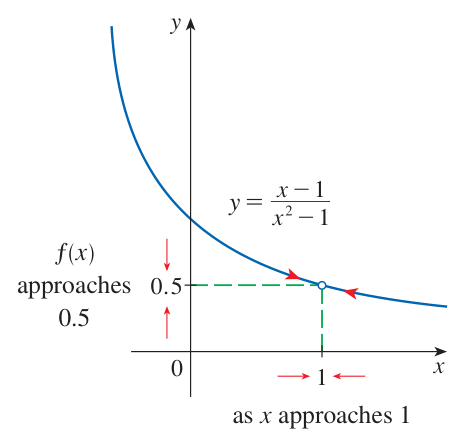
\includegraphics[width=135pt]{images/p0118_fig1.png}\\[5pt]
      {\small\sffamily\bfseries HÌNH 1}
    \end{minipage}%
  }\hspace{20pt}%
}% Từ bảng giá trị và đồ thị của $f$ trong Hình 1, ta thấy rằng khi $x$ càng gần 1 (từ cả hai phía của 1), thì $f(x)$ càng gần 0{,}5. Trên thực tế, có vẻ như ta có thể làm cho các giá trị của $f(x)$ gần 0{,}5 tùy ý bằng cách lấy $x$ đủ gần 1. Ta diễn đạt điều này bằng cách nói “giới hạn của hàm số $f(x) = (x - 1)/(x^2 - 1)$ khi $x$ tiến tới 1 bằng 0{,}5.” Ký hiệu cho điều này là

\begin{equation*}
  \lim_{x \to 1} \frac{x - 1}{x^2 - 1} = 0{,}5
\end{equation*}

\noindent
Tổng quát, chúng ta sử dụng ký hiệu sau.

\begin{tcolorbox}[
  colframe=red!80!black,
  colback=white,
  boxrule=0.8pt,
  arc=0pt,
  left=8pt, right=8pt, top=7pt, bottom=7pt
]
\noindent
\tikz[baseline=-0.55ex]{%
  \node[draw=red!80!black, line width=0.8pt, fill=white, text=red!80!black, font=\bfseries\sffamily\small, inner sep=2pt, minimum size=13pt] {1};%
}\hspace{0.5em}%
{\color{red!80!black}\bfseries\sffamily Định nghĩa trực quan về giới hạn}\quad
Giả sử $f(x)$ được xác định khi $x$ ở gần số $a$. (Điều này có nghĩa là $f$ được xác định trên một khoảng mở nào đó chứa $a$, ngoại trừ có thể tại chính $a$.) Khi đó ta viết
\begin{equation*}
  \lim_{x \to a} f(x) = L
\end{equation*}
\begin{center}
và nói\qquad “giới hạn của $f(x)$, khi $x$ tiến tới $a$, bằng $L$”
\end{center}
nếu ta có thể làm cho các giá trị của $f(x)$ gần $L$ một cách tùy ý (gần $L$ bao nhiêu tùy thích) bằng cách giới hạn $x$ đủ gần $a$ (từ cả hai phía của $a$) nhưng không bằng $a$.
\end{tcolorbox}

\noindent
Nói một cách đại khái, điều này có nghĩa là các giá trị của $f(x)$ tiến dần đến $L$ khi $x$ tiến dần đến $a$. Nói cách khác, các giá trị của $f(x)$ có xu hướng ngày càng gần với số $L$ khi $x$ ngày càng gần với số $a$ (từ cả hai phía của $a$) nhưng $x \neq a$. (Một định nghĩa chính xác hơn sẽ được trình bày trong Mục 2.4.)

\vfill
\begin{center}
\fontsize{5.5}{7}\selectfont\color{gray}
Copyright 2021 Cengage Learning. All Rights Reserved. May not be copied, scanned, or duplicated, in whole or in part. WCN 02-200-203\\
Editorial review has deemed that any suppressed content does not materially affect the overall learning experience. Cengage Learning reserves the right to remove additional content at any time if subsequent rights restrictions require it.
\end{center}
